Scopo dell'esperienza è la stima del calore specifico di un metallo, utilizzando il calorimetro delle mescolanze, altrimenti noto come calorimetro di Regnault. L'esperienza si suddivide in due fasi:
\begin{itemize}
    \item Nella prima fase vine stimata la capacità termica del calorimetro, espressa in termini dell'equivalente in acqua. 
    \item Nella seconda fase viene stimato il calore specifico del metallo la cui composizione è ingota. In questa fase il metallo viene prima riscaldato e poi immerso nel calorimetro contenente acqua a temperatura ambiente.
\end{itemize}
Infine, dal calore specifico del metallo misurato, è stato poi determinato il suo materiale confrontando tale stima con i calori specifici di diverse sostanze.

\begin{figure}[H]
	\centering
	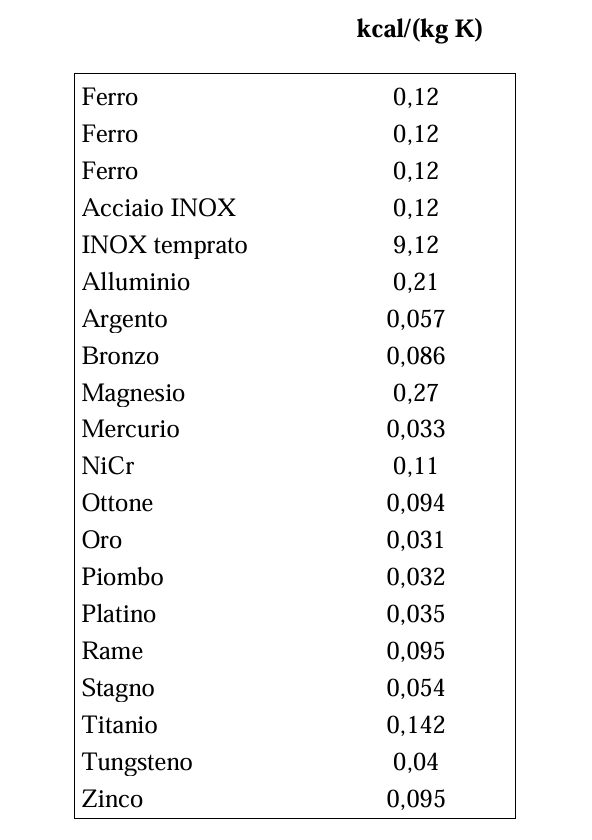
\includegraphics[width=0.44\textwidth]{./figures/materiali}
	\caption{Calori specifici di diversi materiali.}
\end{figure}